\documentclass[a4paper]{book}
\usepackage{a4wide}
\usepackage{makeidx}
\usepackage{graphicx}
\usepackage{multicol}
\usepackage{float}
\usepackage{listings}
\usepackage{color}
\usepackage{textcomp}
\usepackage{alltt}
\usepackage{times}
\usepackage{ifpdf}
\ifpdf
\usepackage[pdftex,
            pagebackref=true,
            colorlinks=true,
            linkcolor=blue,
            unicode
           ]{hyperref}
\else
\usepackage[ps2pdf,
            pagebackref=true,
            colorlinks=true,
            linkcolor=blue,
            unicode
           ]{hyperref}
\usepackage{pspicture}
\fi
\usepackage[utf8]{inputenc}
\usepackage{doxygen}
\lstset{language=C++,inputencoding=utf8,basicstyle=\footnotesize,breaklines=true,breakatwhitespace=true,tabsize=8,numbers=left }
\makeindex
\setcounter{tocdepth}{3}
\renewcommand{\footrulewidth}{0.4pt}
\begin{document}
\hypersetup{pageanchor=false}
\begin{titlepage}
\vspace*{7cm}
\begin{center}
{\Large Reference Manual}\\
\vspace*{1cm}
{\large Generated by Doxygen 1.7.1}\\
\vspace*{0.5cm}
{\small Sun May 6 2012 14:36:31}\\
\end{center}
\end{titlepage}
\clearemptydoublepage
\pagenumbering{roman}
\tableofcontents
\clearemptydoublepage
\pagenumbering{arabic}
\hypersetup{pageanchor=true}
\chapter{Class Index}
\section{Class Hierarchy}
This inheritance list is sorted roughly, but not completely, alphabetically:\begin{DoxyCompactList}
\item \contentsline{section}{BooleanExpression}{\pageref{classBooleanExpression}}{}
\item \contentsline{section}{IsAbleToPlay}{\pageref{interfaceIsAbleToPlay}}{}
\begin{DoxyCompactList}
\item \contentsline{section}{DumbComputerAI}{\pageref{classDumbComputerAI}}{}
\item \contentsline{section}{Human}{\pageref{classHuman}}{}
\end{DoxyCompactList}
\item \contentsline{section}{NimGame}{\pageref{classNimGame}}{}
\item \contentsline{section}{Readable}{\pageref{interfaceReadable}}{}
\begin{DoxyCompactList}
\item \contentsline{section}{Rebus}{\pageref{classRebus}}{}
\end{DoxyCompactList}
\item \contentsline{section}{VectorUtil}{\pageref{classVectorUtil}}{}
\item \contentsline{section}{XOBoard}{\pageref{classXOBoard}}{}
\item \contentsline{section}{XOGame}{\pageref{classXOGame}}{}
\end{DoxyCompactList}

\chapter{Class Index}
\section{Class List}
Here are the classes, structs, unions and interfaces with brief descriptions:\begin{DoxyCompactList}
\item\contentsline{section}{\hyperlink{classBooleanExpression}{BooleanExpression} }{\pageref{classBooleanExpression}}{}
\item\contentsline{section}{\hyperlink{classMaze}{Maze} }{\pageref{classMaze}}{}
\item\contentsline{section}{\hyperlink{classNimGameConf}{NimGameConf} }{\pageref{classNimGameConf}}{}
\item\contentsline{section}{\hyperlink{classRebus}{Rebus} }{\pageref{classRebus}}{}
\item\contentsline{section}{\hyperlink{classSudokuBoard}{SudokuBoard} }{\pageref{classSudokuBoard}}{}
\item\contentsline{section}{\hyperlink{classXOBoard}{XOBoard} }{\pageref{classXOBoard}}{}
\item\contentsline{section}{\hyperlink{classXOGame}{XOGame} }{\pageref{classXOGame}}{}
\end{DoxyCompactList}

\chapter{Class Documentation}
\hypertarget{classBooleanExpression}{
\section{BooleanExpression Class Reference}
\label{classBooleanExpression}\index{BooleanExpression@{BooleanExpression}}
}
\subsection*{Public Member Functions}
\begin{DoxyCompactItemize}
\item 
\hypertarget{classBooleanExpression_add76e02bf45058445aaf70fd6400108c}{
boolean {\bfseries isValid} ()}
\label{classBooleanExpression_add76e02bf45058445aaf70fd6400108c}

\item 
\hypertarget{classBooleanExpression_ae02cb61914b378cdd28cd858d9e8a4a0}{
Lexem\mbox{[}$\,$\mbox{]} {\bfseries getLexems} ()}
\label{classBooleanExpression_ae02cb61914b378cdd28cd858d9e8a4a0}

\end{DoxyCompactItemize}
\subsection*{Package Functions}
\begin{DoxyCompactItemize}
\item 
\hypertarget{classBooleanExpression_a0ac4c6f0eb4d1e9b96bd837aa31de159}{
{\bfseries BooleanExpression} (String stringRepresentation)}
\label{classBooleanExpression_a0ac4c6f0eb4d1e9b96bd837aa31de159}

\end{DoxyCompactItemize}


The documentation for this class was generated from the following file:\begin{DoxyCompactItemize}
\item 
/home/marcvs/Desktop/working/pa-\/materiale/pa/codeBase/Java/src/BooleanExpression.java\end{DoxyCompactItemize}

\hypertarget{classCoord}{
\section{Coord Class Reference}
\label{classCoord}\index{Coord@{Coord}}
}
\subsection*{Public Member Functions}
\begin{DoxyCompactItemize}
\item 
\hypertarget{classCoord_a0ce71339987902b336e340728de4a086}{
{\bfseries Coord} (int lin, int col)}
\label{classCoord_a0ce71339987902b336e340728de4a086}

\end{DoxyCompactItemize}
\subsection*{Public Attributes}
\begin{DoxyCompactItemize}
\item 
\hypertarget{classCoord_a0ab5a34fc4aa09f8cfb1eb7b5536361f}{
int {\bfseries lin}}
\label{classCoord_a0ab5a34fc4aa09f8cfb1eb7b5536361f}

\item 
\hypertarget{classCoord_a7d00b6fb4bfff6fe805b22ff918e21b0}{
int {\bfseries col}}
\label{classCoord_a7d00b6fb4bfff6fe805b22ff918e21b0}

\end{DoxyCompactItemize}
\subsection*{Static Package Attributes}
\begin{DoxyCompactItemize}
\item 
\hypertarget{classCoord_a06f517815dbcd255d655b4b65701a2bf}{
static final \hyperlink{classCoord}{Coord} {\bfseries NOWHERE} = new \hyperlink{classCoord}{Coord}(-\/1, -\/1)}
\label{classCoord_a06f517815dbcd255d655b4b65701a2bf}

\end{DoxyCompactItemize}


The documentation for this class was generated from the following file:\begin{DoxyCompactItemize}
\item 
/home/marcvs/Desktop/working/pa-\/materiale/pa/codeBase/Java/src/Coord.java\end{DoxyCompactItemize}

\hypertarget{classDumbComputerAI}{
\section{DumbComputerAI Class Reference}
\label{classDumbComputerAI}\index{DumbComputerAI@{DumbComputerAI}}
}
Inheritance diagram for DumbComputerAI:\begin{figure}[H]
\begin{center}
\leavevmode
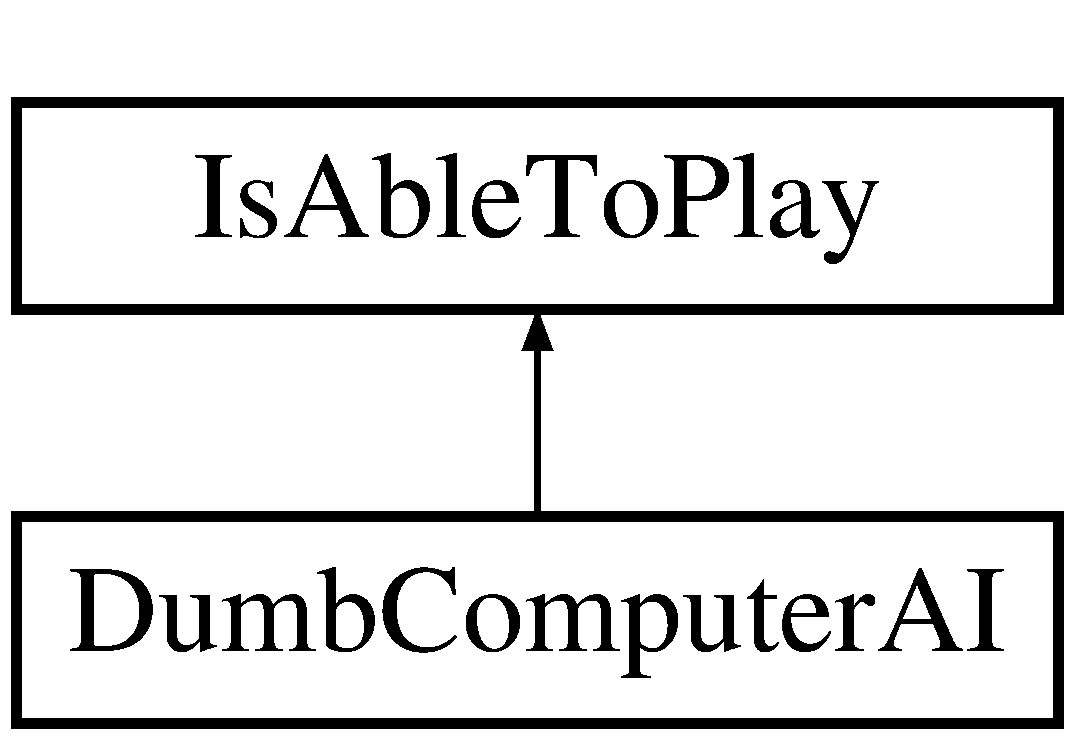
\includegraphics[height=2.000000cm]{classDumbComputerAI}
\end{center}
\end{figure}
\subsection*{Public Member Functions}
\begin{DoxyCompactItemize}
\item 
\hypertarget{classDumbComputerAI_a7cb655ff976f568d859d7f87abf9d36a}{
\hyperlink{classXOBoard}{XOBoard} {\bfseries move} (XOPlayer player, \hyperlink{classXOBoard}{XOBoard} board)}
\label{classDumbComputerAI_a7cb655ff976f568d859d7f87abf9d36a}

\end{DoxyCompactItemize}


The documentation for this class was generated from the following file:\begin{DoxyCompactItemize}
\item 
/home/marcvs/Desktop/working/pa-\/materiale/pa/codeBase/Java/src/XOBoard.java\end{DoxyCompactItemize}

\hypertarget{classGraph}{
\section{Graph Class Reference}
\label{classGraph}\index{Graph@{Graph}}
}
\subsection*{Classes}
\begin{DoxyCompactItemize}
\item 
class {\bfseries Edge}
\end{DoxyCompactItemize}
\subsection*{Public Member Functions}
\begin{DoxyCompactItemize}
\item 
\hypertarget{classGraph_ada3f3f1186255e18b8467b8044a0a45f}{
\hyperlink{classGraph_aa4b8785265efefb668f2931c8f18c8e0}{Graph.Type} {\bfseries getType} ()}
\label{classGraph_ada3f3f1186255e18b8467b8044a0a45f}

\item 
\hyperlink{classGraph_ad807b85e0af693b12607a8f66bdd6f2d}{Graph} (String filename, \hyperlink{classGraph_aa4b8785265efefb668f2931c8f18c8e0}{Graph.Type} type)  throws FileNotFoundException 
\item 
\hypertarget{classGraph_ae06670e180d9bd67674227b1f2a3b8d6}{
{\bfseries Graph} (int size, \hyperlink{classGraph_aa4b8785265efefb668f2931c8f18c8e0}{Graph.Type} type)}
\label{classGraph_ae06670e180d9bd67674227b1f2a3b8d6}

\item 
void \hyperlink{classGraph_a2b4218e18d84fa35a65deb3f92f92b71}{reloadFromDisk} ()  throws FileNotFoundException 
\item 
void \hyperlink{classGraph_a6b0c9ae1efc61d18e9d0850de69007d7}{addEdge} (int x, int y, int c)
\item 
void \hyperlink{classGraph_ac9bac0b67df901c292a6cb7056c1b0d4}{clearParents} ()
\item 
void \hyperlink{classGraph_a84efbb4a0a7fa7f1b9aaa588cb03d454}{setParent} (int node, int parent)
\item 
int \hyperlink{classGraph_af44d0a95f60ebe3a674277f2cc02c339}{getParent} (int node)
\item 
void \hyperlink{classGraph_af3be08d7ab8ae3b8c7d8ea91263eaa20}{printPathBetween} (int first, int last)
\item 
void \hyperlink{classGraph_ae9af916770c65c6b60b582ffc563d8ed}{printAdjMatrix} ()
\item 
void \hyperlink{classGraph_afe6e5a59033d5c3eb35132df7723d8ff}{printCapacityMatrix} ()
\item 
void \hyperlink{classGraph_a7ca9ea178502d458dfe8412856f96342}{printFlowMatrix} ()
\item 
void \hyperlink{classGraph_ac27f2f6fdfad438bfdc73945847c9d35}{printParents} ()
\item 
void \hyperlink{classGraph_ad566bba341395b31350bcc67d43ac858}{printNeighbours} ()
\item 
void \hyperlink{classGraph_aad6e4deef302caff422a47c497e5c6b9}{clearFlow} ()
\item 
void \hyperlink{classGraph_a2ecf3dd3c4897aa924da8e5c221a8509}{print} ()
\item 
\hypertarget{classGraph_ac83f6a4edf0d503d387f59093692d719}{
void {\bfseries printNodes} ()}
\label{classGraph_ac83f6a4edf0d503d387f59093692d719}

\item 
\hypertarget{classGraph_a37a53b4ccf99d9a31976b62b3ab1eea2}{
void {\bfseries printEdges} ()}
\label{classGraph_a37a53b4ccf99d9a31976b62b3ab1eea2}

\item 
int \hyperlink{classGraph_ab7d965333f0ae9e6727676db3224ec4b}{getSize} ()
\item 
boolean \hyperlink{classGraph_ab19bf592d0e75e5863184a1c00c8f52a}{isEdge} (int x, int y)
\item 
\hypertarget{classGraph_aa5a714640bcc1e4c463d7dc8b0a1173c}{
Vector$<$ Integer $>$ {\bfseries getNeighbours} (int node)}
\label{classGraph_aa5a714640bcc1e4c463d7dc8b0a1173c}

\item 
Vector$<$ Edge $>$ \hyperlink{classGraph_a9e1ed7f7e8df8c0fd2be08f09e3da3f0}{getEdges} ()
\item 
Vector$<$ Integer $>$ \hyperlink{classGraph_a57fee445d59d45794cbe606a05c85da7}{getNodes} ()
\end{DoxyCompactItemize}
\subsection*{Public Attributes}
\begin{DoxyCompactItemize}
\item 
boolean\mbox{[}$\,$\mbox{]}\mbox{[}$\,$\mbox{]} \hyperlink{classGraph_a87f661f464d587bc3f6b476c85e800ae}{adjMatrix}
\item 
int\mbox{[}$\,$\mbox{]}\mbox{[}$\,$\mbox{]} \hyperlink{classGraph_a6fe80b61925cedc187fa1ef35c504b1e}{capacityMatrix}
\item 
int\mbox{[}$\,$\mbox{]}\mbox{[}$\,$\mbox{]} \hyperlink{classGraph_ad45717436b6a4ea15d30b88263baeb2a}{flow}
\end{DoxyCompactItemize}
\subsection*{Static Public Attributes}
\begin{DoxyCompactItemize}
\item 
static final int \hyperlink{classGraph_a2dbb2805720a0812f5df6a58d38956af}{UNDEFINED} = Integer.MAX\_\-VALUE
\item 
static final int \hyperlink{classGraph_a282d3ae4575cc3764258ecdb2d8e8fdf}{INFINITY} = Integer.MAX\_\-VALUE
\end{DoxyCompactItemize}
\subsection*{Package Types}
\begin{DoxyCompactItemize}
\item 
enum \hyperlink{classGraph_aa4b8785265efefb668f2931c8f18c8e0}{Type} \{ \hyperlink{classGraph_aa4b8785265efefb668f2931c8f18c8e0}{DIRECTED}, 
\hyperlink{classGraph_aa4b8785265efefb668f2931c8f18c8e0}{UNDIRECTED}
 \}
\end{DoxyCompactItemize}


\subsection{Member Enumeration Documentation}
\hypertarget{classGraph_aa4b8785265efefb668f2931c8f18c8e0}{
\index{Graph@{Graph}!Type@{Type}}
\index{Type@{Type}!Graph@{Graph}}
\subsubsection[{Type}]{\setlength{\rightskip}{0pt plus 5cm}enum {\bf Graph::Type}\hspace{0.3cm}{\ttfamily  \mbox{[}package\mbox{]}}}}
\label{classGraph_aa4b8785265efefb668f2931c8f18c8e0}
\begin{Desc}
\item[Enumerator: ]\par
\begin{description}
\index{DIRECTED@{DIRECTED}!Graph@{Graph}}\index{Graph@{Graph}!DIRECTED@{DIRECTED}}\item[{\em 
\hypertarget{classGraph_aa4b8785265efefb668f2931c8f18c8e0}{
DIRECTED}
\label{classGraph_aa4b8785265efefb668f2931c8f18c8e0}
}]Graf ORIENTAT \index{UNDIRECTED@{UNDIRECTED}!Graph@{Graph}}\index{Graph@{Graph}!UNDIRECTED@{UNDIRECTED}}\item[{\em 
\hypertarget{classGraph_aa4b8785265efefb668f2931c8f18c8e0}{
UNDIRECTED}
\label{classGraph_aa4b8785265efefb668f2931c8f18c8e0}
}]Graf NEOORIENTAT \end{description}
\end{Desc}



\subsection{Constructor \& Destructor Documentation}
\hypertarget{classGraph_ad807b85e0af693b12607a8f66bdd6f2d}{
\index{Graph@{Graph}!Graph@{Graph}}
\index{Graph@{Graph}!Graph@{Graph}}
\subsubsection[{Graph}]{\setlength{\rightskip}{0pt plus 5cm}Graph::Graph (
\begin{DoxyParamCaption}
\item[{String}]{ filename, }
\item[{{\bf Graph.Type}}]{ type}
\end{DoxyParamCaption}
)  throws FileNotFoundException \hspace{0.3cm}{\ttfamily  \mbox{[}inline\mbox{]}}}}
\label{classGraph_ad807b85e0af693b12607a8f66bdd6f2d}

\begin{DoxyParams}{Parameters}
\item[{\em filename}]numele fisierului din care va fi incarcat graful \item[{\em type}]tipul grafului (orientat / neorientat) \end{DoxyParams}


\subsection{Member Function Documentation}
\hypertarget{classGraph_a6b0c9ae1efc61d18e9d0850de69007d7}{
\index{Graph@{Graph}!addEdge@{addEdge}}
\index{addEdge@{addEdge}!Graph@{Graph}}
\subsubsection[{addEdge}]{\setlength{\rightskip}{0pt plus 5cm}void Graph::addEdge (
\begin{DoxyParamCaption}
\item[{int}]{ x, }
\item[{int}]{ y, }
\item[{int}]{ c}
\end{DoxyParamCaption}
)\hspace{0.3cm}{\ttfamily  \mbox{[}inline\mbox{]}}}}
\label{classGraph_a6b0c9ae1efc61d18e9d0850de69007d7}
Adauga un arc de capacitate c intre nodurile x si y. Daca graful este neorientat, va fi adaugat de asemenea si arcul (y, x, c). \hypertarget{classGraph_aad6e4deef302caff422a47c497e5c6b9}{
\index{Graph@{Graph}!clearFlow@{clearFlow}}
\index{clearFlow@{clearFlow}!Graph@{Graph}}
\subsubsection[{clearFlow}]{\setlength{\rightskip}{0pt plus 5cm}void Graph::clearFlow (
\begin{DoxyParamCaption}
{}
\end{DoxyParamCaption}
)\hspace{0.3cm}{\ttfamily  \mbox{[}inline\mbox{]}}}}
\label{classGraph_aad6e4deef302caff422a47c497e5c6b9}
Seteaza toate elementele matricii de flux la 0. \hypertarget{classGraph_ac9bac0b67df901c292a6cb7056c1b0d4}{
\index{Graph@{Graph}!clearParents@{clearParents}}
\index{clearParents@{clearParents}!Graph@{Graph}}
\subsubsection[{clearParents}]{\setlength{\rightskip}{0pt plus 5cm}void Graph::clearParents (
\begin{DoxyParamCaption}
{}
\end{DoxyParamCaption}
)\hspace{0.3cm}{\ttfamily  \mbox{[}inline\mbox{]}}}}
\label{classGraph_ac9bac0b67df901c292a6cb7056c1b0d4}
Initializeaza toti parintii cu \hyperlink{classGraph_a2dbb2805720a0812f5df6a58d38956af}{Graph.UNDEFINED}. \hypertarget{classGraph_a9e1ed7f7e8df8c0fd2be08f09e3da3f0}{
\index{Graph@{Graph}!getEdges@{getEdges}}
\index{getEdges@{getEdges}!Graph@{Graph}}
\subsubsection[{getEdges}]{\setlength{\rightskip}{0pt plus 5cm}Vector$<$Edge$>$ Graph::getEdges (
\begin{DoxyParamCaption}
{}
\end{DoxyParamCaption}
)\hspace{0.3cm}{\ttfamily  \mbox{[}inline\mbox{]}}}}
\label{classGraph_a9e1ed7f7e8df8c0fd2be08f09e3da3f0}
Intoarce un vector cu toate muchiile din graf. \hypertarget{classGraph_a57fee445d59d45794cbe606a05c85da7}{
\index{Graph@{Graph}!getNodes@{getNodes}}
\index{getNodes@{getNodes}!Graph@{Graph}}
\subsubsection[{getNodes}]{\setlength{\rightskip}{0pt plus 5cm}Vector$<$Integer$>$ Graph::getNodes (
\begin{DoxyParamCaption}
{}
\end{DoxyParamCaption}
)\hspace{0.3cm}{\ttfamily  \mbox{[}inline\mbox{]}}}}
\label{classGraph_a57fee445d59d45794cbe606a05c85da7}
Intoarce un vector cu toate nodurile din graf pentru a putea fi folosit (de exemplu) intr-\/o constructie precum \char`\"{}for(int k : graph.getNodes())\char`\"{}. \hypertarget{classGraph_af44d0a95f60ebe3a674277f2cc02c339}{
\index{Graph@{Graph}!getParent@{getParent}}
\index{getParent@{getParent}!Graph@{Graph}}
\subsubsection[{getParent}]{\setlength{\rightskip}{0pt plus 5cm}int Graph::getParent (
\begin{DoxyParamCaption}
\item[{int}]{ node}
\end{DoxyParamCaption}
)\hspace{0.3cm}{\ttfamily  \mbox{[}inline\mbox{]}}}}
\label{classGraph_af44d0a95f60ebe3a674277f2cc02c339}
Intoarce parintele unui anumit nod sau \hyperlink{classGraph_a2dbb2805720a0812f5df6a58d38956af}{Graph.UNDEFINED} daca acesta nu a fost setat. \hypertarget{classGraph_ab7d965333f0ae9e6727676db3224ec4b}{
\index{Graph@{Graph}!getSize@{getSize}}
\index{getSize@{getSize}!Graph@{Graph}}
\subsubsection[{getSize}]{\setlength{\rightskip}{0pt plus 5cm}int Graph::getSize (
\begin{DoxyParamCaption}
{}
\end{DoxyParamCaption}
)\hspace{0.3cm}{\ttfamily  \mbox{[}inline\mbox{]}}}}
\label{classGraph_ab7d965333f0ae9e6727676db3224ec4b}
Intoarce numarul de noduri din graf. \hypertarget{classGraph_ab19bf592d0e75e5863184a1c00c8f52a}{
\index{Graph@{Graph}!isEdge@{isEdge}}
\index{isEdge@{isEdge}!Graph@{Graph}}
\subsubsection[{isEdge}]{\setlength{\rightskip}{0pt plus 5cm}boolean Graph::isEdge (
\begin{DoxyParamCaption}
\item[{int}]{ x, }
\item[{int}]{ y}
\end{DoxyParamCaption}
)\hspace{0.3cm}{\ttfamily  \mbox{[}inline\mbox{]}}}}
\label{classGraph_ab19bf592d0e75e5863184a1c00c8f52a}
Intoarce true in cazul in care intre nodurile date ca parametru exista muchie si false in caz contrar. \hypertarget{classGraph_a2ecf3dd3c4897aa924da8e5c221a8509}{
\index{Graph@{Graph}!print@{print}}
\index{print@{print}!Graph@{Graph}}
\subsubsection[{print}]{\setlength{\rightskip}{0pt plus 5cm}void Graph::print (
\begin{DoxyParamCaption}
{}
\end{DoxyParamCaption}
)\hspace{0.3cm}{\ttfamily  \mbox{[}inline\mbox{]}}}}
\label{classGraph_a2ecf3dd3c4897aa924da8e5c221a8509}
Afiseaza toate informatiile despre graf \hypertarget{classGraph_ae9af916770c65c6b60b582ffc563d8ed}{
\index{Graph@{Graph}!printAdjMatrix@{printAdjMatrix}}
\index{printAdjMatrix@{printAdjMatrix}!Graph@{Graph}}
\subsubsection[{printAdjMatrix}]{\setlength{\rightskip}{0pt plus 5cm}void Graph::printAdjMatrix (
\begin{DoxyParamCaption}
{}
\end{DoxyParamCaption}
)\hspace{0.3cm}{\ttfamily  \mbox{[}inline\mbox{]}}}}
\label{classGraph_ae9af916770c65c6b60b582ffc563d8ed}
Afiseaza matricea de adiacenta asociata grafului. \hypertarget{classGraph_afe6e5a59033d5c3eb35132df7723d8ff}{
\index{Graph@{Graph}!printCapacityMatrix@{printCapacityMatrix}}
\index{printCapacityMatrix@{printCapacityMatrix}!Graph@{Graph}}
\subsubsection[{printCapacityMatrix}]{\setlength{\rightskip}{0pt plus 5cm}void Graph::printCapacityMatrix (
\begin{DoxyParamCaption}
{}
\end{DoxyParamCaption}
)\hspace{0.3cm}{\ttfamily  \mbox{[}inline\mbox{]}}}}
\label{classGraph_afe6e5a59033d5c3eb35132df7723d8ff}
Afiseaza matricea de capacitati asociata grafului. \hypertarget{classGraph_a7ca9ea178502d458dfe8412856f96342}{
\index{Graph@{Graph}!printFlowMatrix@{printFlowMatrix}}
\index{printFlowMatrix@{printFlowMatrix}!Graph@{Graph}}
\subsubsection[{printFlowMatrix}]{\setlength{\rightskip}{0pt plus 5cm}void Graph::printFlowMatrix (
\begin{DoxyParamCaption}
{}
\end{DoxyParamCaption}
)\hspace{0.3cm}{\ttfamily  \mbox{[}inline\mbox{]}}}}
\label{classGraph_a7ca9ea178502d458dfe8412856f96342}
Afiseaza matricea de flux asociata grafului. \hypertarget{classGraph_ad566bba341395b31350bcc67d43ac858}{
\index{Graph@{Graph}!printNeighbours@{printNeighbours}}
\index{printNeighbours@{printNeighbours}!Graph@{Graph}}
\subsubsection[{printNeighbours}]{\setlength{\rightskip}{0pt plus 5cm}void Graph::printNeighbours (
\begin{DoxyParamCaption}
{}
\end{DoxyParamCaption}
)\hspace{0.3cm}{\ttfamily  \mbox{[}inline\mbox{]}}}}
\label{classGraph_ad566bba341395b31350bcc67d43ac858}
Afiseaza graful sub forma de liste de adiacenta (fiecare nod este urmat de vecinii sai). \hypertarget{classGraph_ac27f2f6fdfad438bfdc73945847c9d35}{
\index{Graph@{Graph}!printParents@{printParents}}
\index{printParents@{printParents}!Graph@{Graph}}
\subsubsection[{printParents}]{\setlength{\rightskip}{0pt plus 5cm}void Graph::printParents (
\begin{DoxyParamCaption}
{}
\end{DoxyParamCaption}
)\hspace{0.3cm}{\ttfamily  \mbox{[}inline\mbox{]}}}}
\label{classGraph_ac27f2f6fdfad438bfdc73945847c9d35}
Afiseaza vectorul de parinti. \hypertarget{classGraph_af3be08d7ab8ae3b8c7d8ea91263eaa20}{
\index{Graph@{Graph}!printPathBetween@{printPathBetween}}
\index{printPathBetween@{printPathBetween}!Graph@{Graph}}
\subsubsection[{printPathBetween}]{\setlength{\rightskip}{0pt plus 5cm}void Graph::printPathBetween (
\begin{DoxyParamCaption}
\item[{int}]{ first, }
\item[{int}]{ last}
\end{DoxyParamCaption}
)\hspace{0.3cm}{\ttfamily  \mbox{[}inline\mbox{]}}}}
\label{classGraph_af3be08d7ab8ae3b8c7d8ea91263eaa20}
Tipareste calea intre doua noduri. Este necesar ca, in prealabil, sa fi fost folosita functia \hyperlink{classGraph_a84efbb4a0a7fa7f1b9aaa588cb03d454}{setParent()} pentru a seta corect parintii.


\begin{DoxyParams}{Parameters}
\item[{\em first}]nodul sursa \item[{\em last}]nodul destinatie \end{DoxyParams}
\hypertarget{classGraph_a2b4218e18d84fa35a65deb3f92f92b71}{
\index{Graph@{Graph}!reloadFromDisk@{reloadFromDisk}}
\index{reloadFromDisk@{reloadFromDisk}!Graph@{Graph}}
\subsubsection[{reloadFromDisk}]{\setlength{\rightskip}{0pt plus 5cm}void Graph::reloadFromDisk (
\begin{DoxyParamCaption}
{}
\end{DoxyParamCaption}
)  throws FileNotFoundException \hspace{0.3cm}{\ttfamily  \mbox{[}inline\mbox{]}}}}
\label{classGraph_a2b4218e18d84fa35a65deb3f92f92b71}
Reconstruieste graful folosind aceiasi paramentri din constructor.

Functia poate fi chemata pentru a reseta graful la starea initiala. \hypertarget{classGraph_a84efbb4a0a7fa7f1b9aaa588cb03d454}{
\index{Graph@{Graph}!setParent@{setParent}}
\index{setParent@{setParent}!Graph@{Graph}}
\subsubsection[{setParent}]{\setlength{\rightskip}{0pt plus 5cm}void Graph::setParent (
\begin{DoxyParamCaption}
\item[{int}]{ node, }
\item[{int}]{ parent}
\end{DoxyParamCaption}
)\hspace{0.3cm}{\ttfamily  \mbox{[}inline\mbox{]}}}}
\label{classGraph_a84efbb4a0a7fa7f1b9aaa588cb03d454}
Retine pe \char`\"{}parent\char`\"{} drept parintele lui \char`\"{}node\char`\"{}.


\begin{DoxyParams}{Parameters}
\item[{\em node}]nodul pe al carui parinte vrem sa il setam \item[{\em parent}]parintele nodului \end{DoxyParams}


\subsection{Member Data Documentation}
\hypertarget{classGraph_a87f661f464d587bc3f6b476c85e800ae}{
\index{Graph@{Graph}!adjMatrix@{adjMatrix}}
\index{adjMatrix@{adjMatrix}!Graph@{Graph}}
\subsubsection[{adjMatrix}]{\setlength{\rightskip}{0pt plus 5cm}boolean \mbox{[}$\,$\mbox{]}\mbox{[}$\,$\mbox{]} {\bf Graph::adjMatrix}}}
\label{classGraph_a87f661f464d587bc3f6b476c85e800ae}
Matricea de adiacenta asociata grafului.

adjMatrix\mbox{[}x\mbox{]}\mbox{[}y\mbox{]} == true $<$=$>$ exista un arc de la nodul \char`\"{}x\char`\"{} la nodul \char`\"{}y\char`\"{} \hypertarget{classGraph_a6fe80b61925cedc187fa1ef35c504b1e}{
\index{Graph@{Graph}!capacityMatrix@{capacityMatrix}}
\index{capacityMatrix@{capacityMatrix}!Graph@{Graph}}
\subsubsection[{capacityMatrix}]{\setlength{\rightskip}{0pt plus 5cm}int \mbox{[}$\,$\mbox{]}\mbox{[}$\,$\mbox{]} {\bf Graph::capacityMatrix}}}
\label{classGraph_a6fe80b61925cedc187fa1ef35c504b1e}
Matricea de capacitati asociata grafului.

capacityMatrix\mbox{[}x\mbox{]}\mbox{[}y\mbox{]} == capacitatea asociata arcului de la nodul \char`\"{}x\char`\"{} la nodul \char`\"{}y\char`\"{} \hypertarget{classGraph_ad45717436b6a4ea15d30b88263baeb2a}{
\index{Graph@{Graph}!flow@{flow}}
\index{flow@{flow}!Graph@{Graph}}
\subsubsection[{flow}]{\setlength{\rightskip}{0pt plus 5cm}int \mbox{[}$\,$\mbox{]}\mbox{[}$\,$\mbox{]} {\bf Graph::flow}}}
\label{classGraph_ad45717436b6a4ea15d30b88263baeb2a}
Matricea de flux asociata grafului (poate fi folosita pentru a retine fluxul transportat de retea).

flow\mbox{[}x\mbox{]}\mbox{[}y\mbox{]} == fluxul asociat arcului de la nodul \char`\"{}x\char`\"{} la nodul \char`\"{}y\char`\"{} \hypertarget{classGraph_a282d3ae4575cc3764258ecdb2d8e8fdf}{
\index{Graph@{Graph}!INFINITY@{INFINITY}}
\index{INFINITY@{INFINITY}!Graph@{Graph}}
\subsubsection[{INFINITY}]{\setlength{\rightskip}{0pt plus 5cm}final int {\bf Graph::INFINITY} = Integer.MAX\_\-VALUE\hspace{0.3cm}{\ttfamily  \mbox{[}static\mbox{]}}}}
\label{classGraph_a282d3ae4575cc3764258ecdb2d8e8fdf}
INIFINIT \hypertarget{classGraph_a2dbb2805720a0812f5df6a58d38956af}{
\index{Graph@{Graph}!UNDEFINED@{UNDEFINED}}
\index{UNDEFINED@{UNDEFINED}!Graph@{Graph}}
\subsubsection[{UNDEFINED}]{\setlength{\rightskip}{0pt plus 5cm}final int {\bf Graph::UNDEFINED} = Integer.MAX\_\-VALUE\hspace{0.3cm}{\ttfamily  \mbox{[}static\mbox{]}}}}
\label{classGraph_a2dbb2805720a0812f5df6a58d38956af}
NEDEFINIT 

The documentation for this class was generated from the following file:\begin{DoxyCompactItemize}
\item 
/home/marcvs/Desktop/working/pa-\/materiale/pa/codeBase/Java/src/Graph.java\end{DoxyCompactItemize}

\hypertarget{classHuman}{
\section{Human Class Reference}
\label{classHuman}\index{Human@{Human}}
}
Inheritance diagram for Human:\begin{figure}[H]
\begin{center}
\leavevmode
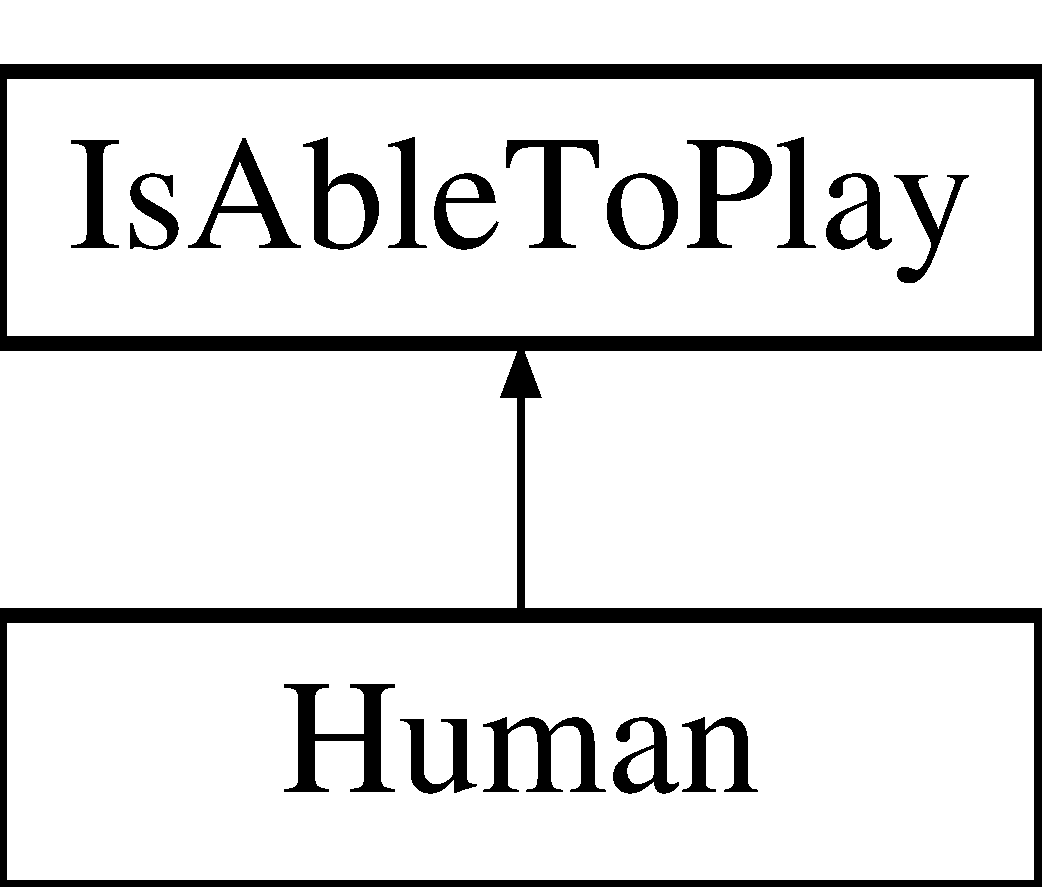
\includegraphics[height=2.000000cm]{classHuman}
\end{center}
\end{figure}
\subsection*{Public Member Functions}
\begin{DoxyCompactItemize}
\item 
\hypertarget{classHuman_a23e90c0545d898da0d16f716d1cdbeb1}{
\hyperlink{classXOBoard}{XOBoard} {\bfseries move} (XOPlayer player, \hyperlink{classXOBoard}{XOBoard} board)}
\label{classHuman_a23e90c0545d898da0d16f716d1cdbeb1}

\end{DoxyCompactItemize}


The documentation for this class was generated from the following file:\begin{DoxyCompactItemize}
\item 
/home/marcvs/Desktop/working/pa-\/materiale/pa/codeBase/Java/src/XOBoard.java\end{DoxyCompactItemize}

\hypertarget{interfaceIsAbleToPlay}{
\section{IsAbleToPlay Interface Reference}
\label{interfaceIsAbleToPlay}\index{IsAbleToPlay@{IsAbleToPlay}}
}
Inheritance diagram for IsAbleToPlay:\begin{figure}[H]
\begin{center}
\leavevmode
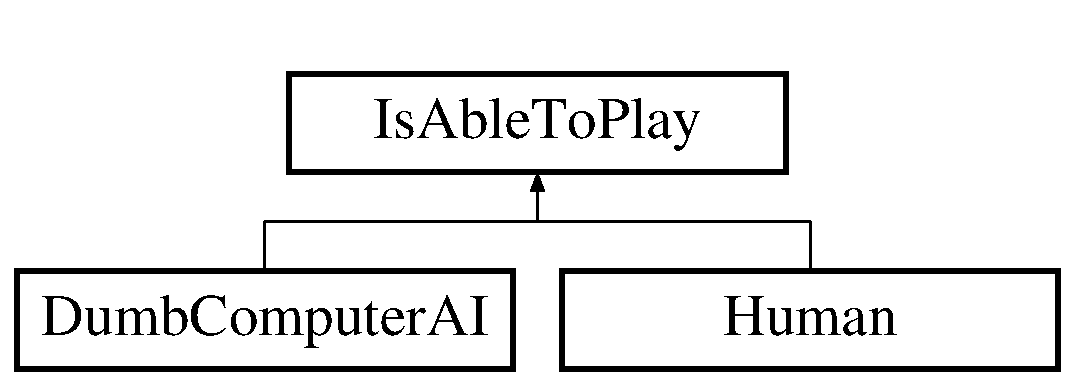
\includegraphics[height=2.000000cm]{interfaceIsAbleToPlay}
\end{center}
\end{figure}
\subsection*{Public Member Functions}
\begin{DoxyCompactItemize}
\item 
\hypertarget{interfaceIsAbleToPlay_ade65fcb1c3423d01bdd059e5ccd22a6d}{
\hyperlink{classXOBoard}{XOBoard} {\bfseries move} (XOPlayer player, \hyperlink{classXOBoard}{XOBoard} board)}
\label{interfaceIsAbleToPlay_ade65fcb1c3423d01bdd059e5ccd22a6d}

\end{DoxyCompactItemize}


The documentation for this interface was generated from the following file:\begin{DoxyCompactItemize}
\item 
/home/marcvs/Desktop/working/pa-\/materiale/pa/codeBase/Java/src/XOBoard.java\end{DoxyCompactItemize}

\hypertarget{classMaze}{
\section{Maze Class Reference}
\label{classMaze}\index{Maze@{Maze}}
}
Inheritance diagram for Maze:\begin{figure}[H]
\begin{center}
\leavevmode
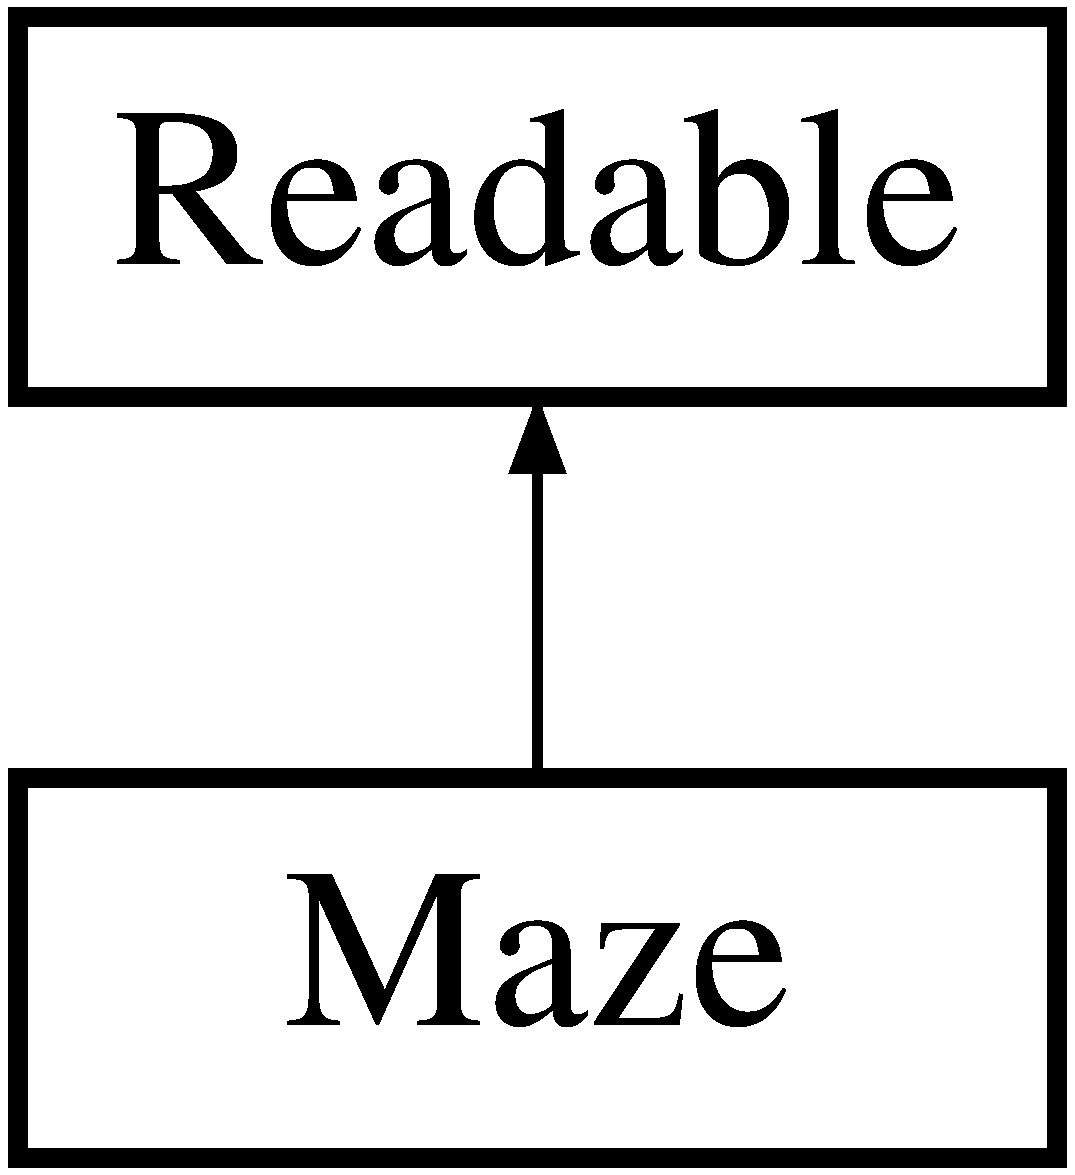
\includegraphics[height=2.000000cm]{classMaze}
\end{center}
\end{figure}
\subsection*{Public Member Functions}
\begin{DoxyCompactItemize}
\item 
\hypertarget{classMaze_a8f1cc7d8dd3fa426ace16bf32f54f24f}{
{\bfseries Maze} (int height, int width)}
\label{classMaze_a8f1cc7d8dd3fa426ace16bf32f54f24f}

\item 
\hypertarget{classMaze_a3f9b79edb99a9726da62bc6823ea9149}{
int {\bfseries get\_\-width} ()}
\label{classMaze_a3f9b79edb99a9726da62bc6823ea9149}

\item 
\hypertarget{classMaze_a43a3408e506b2f2463fc985865b3c850}{
int {\bfseries get\_\-height} ()}
\label{classMaze_a43a3408e506b2f2463fc985865b3c850}

\item 
\hypertarget{classMaze_a18724de009238efe119be4c80906416f}{
boolean {\bfseries is\_\-walkable} (int line, int column)}
\label{classMaze_a18724de009238efe119be4c80906416f}

\item 
\hypertarget{classMaze_a1156760e57f75cd36241a9244f902277}{
boolean {\bfseries is\_\-walkable} (\hyperlink{classCoord}{Coord} coord)}
\label{classMaze_a1156760e57f75cd36241a9244f902277}

\item 
\hypertarget{classMaze_ac223c8189bee28e047d4399cff5fa765}{
boolean {\bfseries is\_\-exit\_\-point} (int line, int column)}
\label{classMaze_ac223c8189bee28e047d4399cff5fa765}

\item 
\hypertarget{classMaze_a5ee98f5633093dc2e1cba6c03e4ddb54}{
boolean {\bfseries is\_\-exit\_\-point} (\hyperlink{classCoord}{Coord} coord)}
\label{classMaze_a5ee98f5633093dc2e1cba6c03e4ddb54}

\item 
\hypertarget{classMaze_a258ccfd950d62359774ed00a75591eaa}{
void {\bfseries mark\_\-solution\_\-step} (int line, int column)}
\label{classMaze_a258ccfd950d62359774ed00a75591eaa}

\item 
\hypertarget{classMaze_a0b27a912b886cd33a45d53789e4f2f1b}{
void {\bfseries mark\_\-solution\_\-step} (\hyperlink{classCoord}{Coord} coord)}
\label{classMaze_a0b27a912b886cd33a45d53789e4f2f1b}

\item 
\hypertarget{classMaze_a70725da73e2032a640bd80db1a51b1dc}{
void {\bfseries read} (Scanner scanner)}
\label{classMaze_a70725da73e2032a640bd80db1a51b1dc}

\item 
\hypertarget{classMaze_a6eb47c884e545475598f784707088f8b}{
void {\bfseries print} ()}
\label{classMaze_a6eb47c884e545475598f784707088f8b}

\end{DoxyCompactItemize}


The documentation for this class was generated from the following file:\begin{DoxyCompactItemize}
\item 
/home/marcvs/Desktop/working/pa-\/materiale/pa/codeBase/Java/src/Maze.java\end{DoxyCompactItemize}

\hypertarget{classNimGame}{
\section{NimGame Class Reference}
\label{classNimGame}\index{NimGame@{NimGame}}
}
\subsection*{Public Member Functions}
\begin{DoxyCompactItemize}
\item 
\hypertarget{classNimGame_a8543bfe2b34632f4c94977cb62637e33}{
{\bfseries NimGame} (int n)}
\label{classNimGame_a8543bfe2b34632f4c94977cb62637e33}

\item 
\hypertarget{classNimGame_af1c40e64cf13a03ef237ccb04a9e14df}{
int {\bfseries size} ()}
\label{classNimGame_af1c40e64cf13a03ef237ccb04a9e14df}

\item 
\hypertarget{classNimGame_ab53242c239178356333cd8621ef17e3e}{
boolean {\bfseries gameOver} ()}
\label{classNimGame_ab53242c239178356333cd8621ef17e3e}

\item 
\hypertarget{classNimGame_a77f7701745e5b67a695dfbdc8ea32e9e}{
int {\bfseries get} (int index)}
\label{classNimGame_a77f7701745e5b67a695dfbdc8ea32e9e}

\item 
\hypertarget{classNimGame_a63b153aa9874dfe8e2d8bd486143a015}{
void {\bfseries split} (int heap, int a, int b)}
\label{classNimGame_a63b153aa9874dfe8e2d8bd486143a015}

\item 
\hypertarget{classNimGame_a7e8904a911442a899d1420b1ea913f01}{
void {\bfseries unsplit} (int heap, int a, int b)}
\label{classNimGame_a7e8904a911442a899d1420b1ea913f01}

\item 
\hypertarget{classNimGame_a1ab91c05860dd790a8fc2e0f35fbb00a}{
void {\bfseries print} ()}
\label{classNimGame_a1ab91c05860dd790a8fc2e0f35fbb00a}

\end{DoxyCompactItemize}


The documentation for this class was generated from the following file:\begin{DoxyCompactItemize}
\item 
/home/marcvs/Desktop/working/pa-\/materiale/pa/codeBase/Java/src/NimGame.java\end{DoxyCompactItemize}

\hypertarget{interfaceReadable}{
\section{Readable Interface Reference}
\label{interfaceReadable}\index{Readable@{Readable}}
}
Inheritance diagram for Readable:\begin{figure}[H]
\begin{center}
\leavevmode
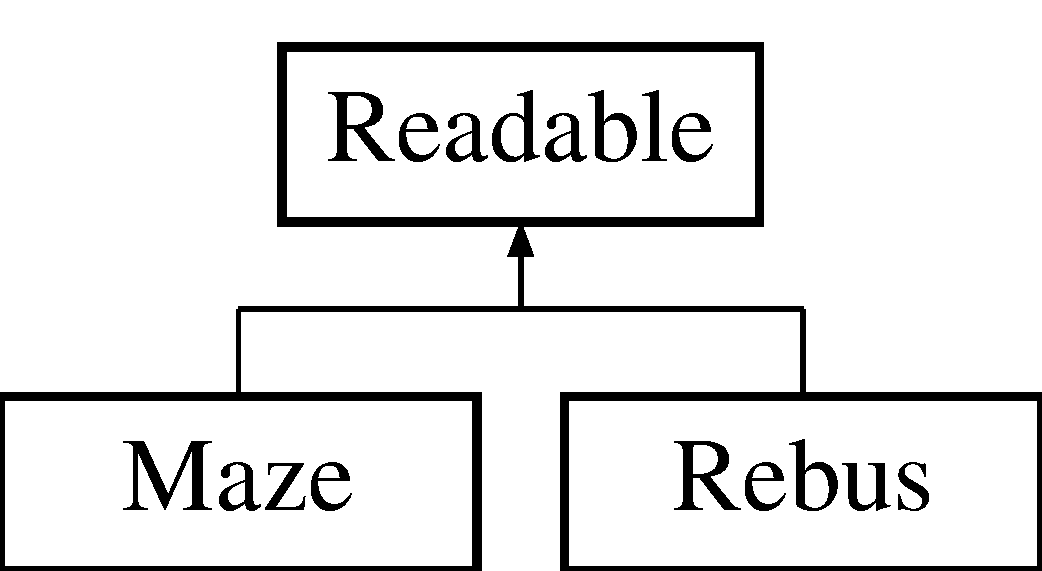
\includegraphics[height=2.000000cm]{interfaceReadable}
\end{center}
\end{figure}
\subsection*{Public Member Functions}
\begin{DoxyCompactItemize}
\item 
\hypertarget{interfaceReadable_a4ff1529890f69b2ad321bc06e497ed16}{
void {\bfseries read} (Scanner scanner)}
\label{interfaceReadable_a4ff1529890f69b2ad321bc06e497ed16}

\end{DoxyCompactItemize}


The documentation for this interface was generated from the following file:\begin{DoxyCompactItemize}
\item 
/home/marcvs/Desktop/working/pa-\/materiale/pa/codeBase/Java/src/Readable.java\end{DoxyCompactItemize}

\hypertarget{classRebus}{
\section{Rebus Class Reference}
\label{classRebus}\index{Rebus@{Rebus}}
}
Inheritance diagram for Rebus:\begin{figure}[H]
\begin{center}
\leavevmode
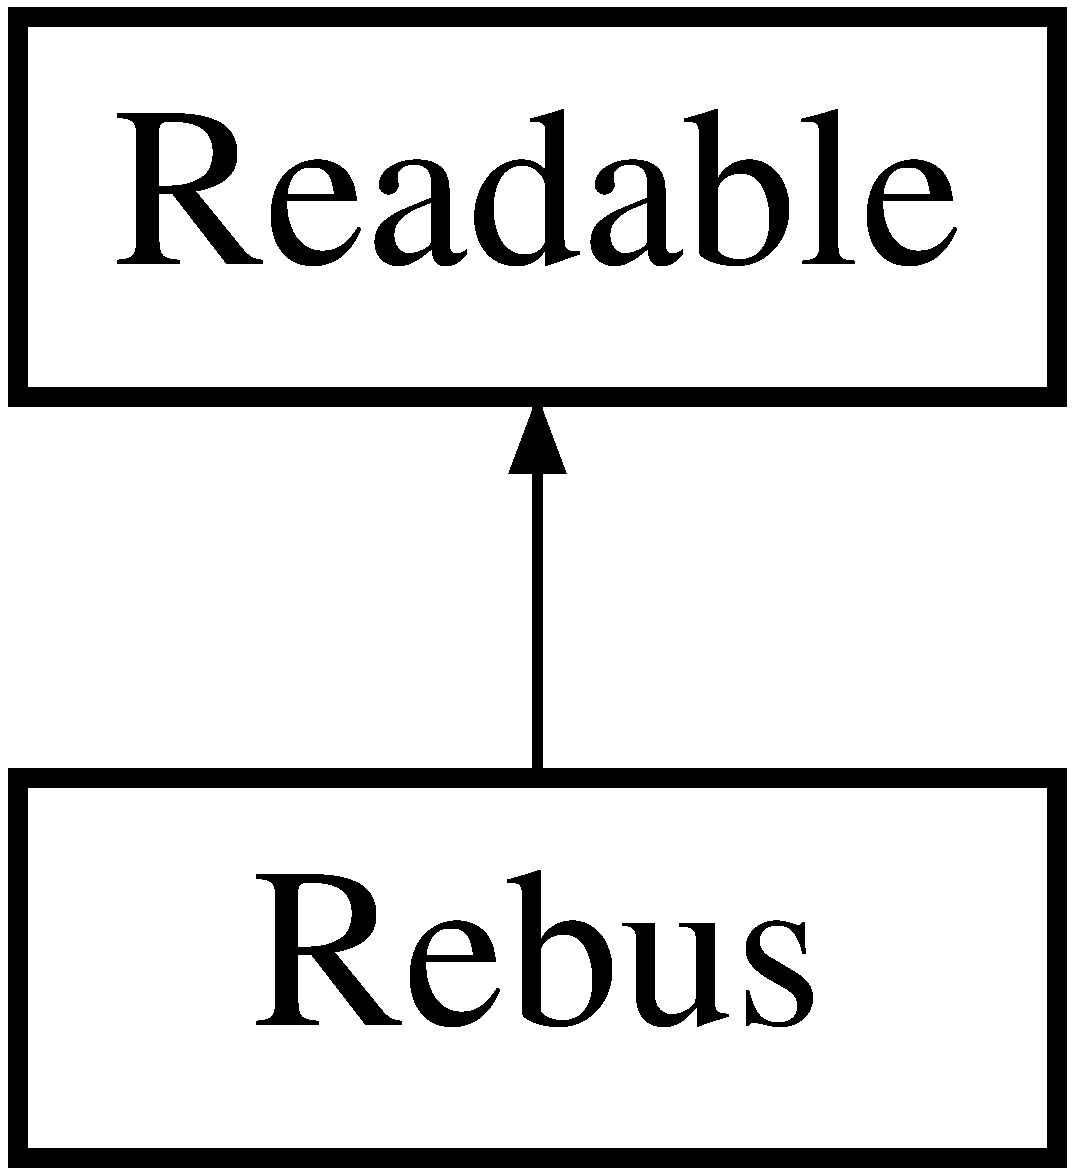
\includegraphics[height=2.000000cm]{classRebus}
\end{center}
\end{figure}
\subsection*{Public Member Functions}
\begin{DoxyCompactItemize}
\item 
\hypertarget{classRebus_a2495b8ab66b8b5fc73be661e6ccb85d3}{
char {\bfseries get} (int row, int column)}
\label{classRebus_a2495b8ab66b8b5fc73be661e6ccb85d3}

\item 
\hypertarget{classRebus_a33c68ead613e1cad7e1e274451f769c0}{
void {\bfseries put} (int row, int column, char c)}
\label{classRebus_a33c68ead613e1cad7e1e274451f769c0}

\item 
\hypertarget{classRebus_ab1ffa625317a5f6f05c75ec072a4bf53}{
void {\bfseries read} (Scanner scanner)}
\label{classRebus_ab1ffa625317a5f6f05c75ec072a4bf53}

\item 
\hypertarget{classRebus_ad208ddcbae9a498c5e8ef2beec2a3306}{
String {\bfseries toString} ()}
\label{classRebus_ad208ddcbae9a498c5e8ef2beec2a3306}

\end{DoxyCompactItemize}
\subsection*{Public Attributes}
\begin{DoxyCompactItemize}
\item 
\hypertarget{classRebus_a0d21b9515af691a04c515a3c163bd683}{
int {\bfseries rows}}
\label{classRebus_a0d21b9515af691a04c515a3c163bd683}

\item 
\hypertarget{classRebus_a71ec10584853e625028ea0c7c4932256}{
int {\bfseries columns}}
\label{classRebus_a71ec10584853e625028ea0c7c4932256}

\end{DoxyCompactItemize}
\subsection*{Package Functions}
\begin{DoxyCompactItemize}
\item 
\hypertarget{classRebus_ae7febf865939cb84fc08a087d12ee465}{
void {\bfseries putString} (int row, int column, String s)}
\label{classRebus_ae7febf865939cb84fc08a087d12ee465}

\item 
\hypertarget{classRebus_a7f568be5d10645247a9c3b9c3aefd31b}{
void {\bfseries eraseString} (int row, int column)}
\label{classRebus_a7f568be5d10645247a9c3b9c3aefd31b}

\item 
\hypertarget{classRebus_a51b184a4ff31ffb8d696daf86b6027f9}{
void {\bfseries erase} (int row, int column)}
\label{classRebus_a51b184a4ff31ffb8d696daf86b6027f9}

\item 
\hypertarget{classRebus_ad429f688c0bd500988843f21426bca97}{
boolean {\bfseries is\_\-empty} (int row, int column)}
\label{classRebus_ad429f688c0bd500988843f21426bca97}

\item 
\hypertarget{classRebus_a75a4903e5f1d6ecb72c3689fda4422f3}{
boolean {\bfseries is\_\-done} ()}
\label{classRebus_a75a4903e5f1d6ecb72c3689fda4422f3}

\end{DoxyCompactItemize}
\subsection*{Package Attributes}
\begin{DoxyCompactItemize}
\item 
\hypertarget{classRebus_aa874c93e563860b32ee8d70bd15b66c7}{
char\mbox{[}$\,$\mbox{]}\mbox{[}$\,$\mbox{]} {\bfseries m}}
\label{classRebus_aa874c93e563860b32ee8d70bd15b66c7}

\item 
\hypertarget{classRebus_a3279788d9a6d47b8c7bc6857582d298c}{
char\mbox{[}$\,$\mbox{]}\mbox{[}$\,$\mbox{]} {\bfseries ref}}
\label{classRebus_a3279788d9a6d47b8c7bc6857582d298c}

\end{DoxyCompactItemize}


The documentation for this class was generated from the following file:\begin{DoxyCompactItemize}
\item 
/home/marcvs/Desktop/working/pa-\/materiale/pa/codeBase/Java/src/Rebus.java\end{DoxyCompactItemize}

\hypertarget{classVectorUtil}{
\section{VectorUtil Class Reference}
\label{classVectorUtil}\index{VectorUtil@{VectorUtil}}
}
\subsection*{Static Public Member Functions}
\begin{DoxyCompactItemize}
\item 
\hypertarget{classVectorUtil_aff4c2878342ce74cd1dbed299fa16678}{
static$<$ T $>$ T\mbox{[}$\,$\mbox{]} {\bfseries readArrayOfReadables} (T\mbox{[}$\,$\mbox{]} vectorHint, Class classType)}
\label{classVectorUtil_aff4c2878342ce74cd1dbed299fa16678}

\item 
\hypertarget{classVectorUtil_a872045ae05e75378562d354bf14df5dd}{
static int\mbox{[}$\,$\mbox{]} {\bfseries readArrayOfIntegers} ()}
\label{classVectorUtil_a872045ae05e75378562d354bf14df5dd}

\end{DoxyCompactItemize}


The documentation for this class was generated from the following file:\begin{DoxyCompactItemize}
\item 
/home/marcvs/Desktop/working/pa-\/materiale/pa/codeBase/Java/src/VectorUtil.java\end{DoxyCompactItemize}

\hypertarget{classXOBoard}{
\section{XOBoard Class Reference}
\label{classXOBoard}\index{XOBoard@{XOBoard}}
}
\subsection*{Public Types}
\begin{DoxyCompactItemize}
\item 
enum {\bfseries Player} \{ {\bfseries PlayerX}, 
{\bfseries PlayerO}
 \}
\end{DoxyCompactItemize}
\subsection*{Public Member Functions}
\begin{DoxyCompactItemize}
\item 
\hypertarget{classXOBoard_a5740df9f6637e64adb7745228820b608}{
\hyperlink{classXOBoard_a5740df9f6637e64adb7745228820b608}{XOBoard} ()}
\label{classXOBoard_a5740df9f6637e64adb7745228820b608}

\begin{DoxyCompactList}\small\item\em Constructor fara parametri care instantiaza o tabla goala pe care nu este marcat nimic. \item\end{DoxyCompactList}\item 
bool \hyperlink{classXOBoard_afc284df051b707b824bc8289e5bffd22}{is\_\-empty} (int x, int y) const 
\begin{DoxyCompactList}\small\item\em Metoda care verifica daca o celula este libera sau nu. \item\end{DoxyCompactList}\item 
char \hyperlink{classXOBoard_a850b7cbdb93c080eb7db8d749bf1aafa}{get} (int x, int y) const 
\begin{DoxyCompactList}\small\item\em Metoda care intoarce caracterul de pe tabla. \item\end{DoxyCompactList}\item 
void \hyperlink{classXOBoard_a3190b1cd4b6d1665bb0b6c35411d0c3e}{put} (Player player, int x, int y)
\begin{DoxyCompactList}\small\item\em Metoda care bifeaza o celula de pe tabla in numele unui jucator. \item\end{DoxyCompactList}\item 
void \hyperlink{classXOBoard_a6e72af673a48b7a4de79d7b738a690c1}{erase} (int x, int y)
\begin{DoxyCompactList}\small\item\em Metoda care sterge valoarea dintr-\/o celula de pe tabla. \item\end{DoxyCompactList}\item 
bool \hyperlink{classXOBoard_a58b290b18786b246c9051958819b1d4f}{is\_\-full} () const 
\begin{DoxyCompactList}\small\item\em Metoda care spune daca tabla s-\/a terminat de completat sau nu. \item\end{DoxyCompactList}\item 
int \hyperlink{classXOBoard_a8affd589eb32be52b4a58cdb487eaee5}{get\_\-score} (Player player) const 
\begin{DoxyCompactList}\small\item\em Metoda care intoarce scorul tablei din perspectiva jucatorului dat ca parametru. \item\end{DoxyCompactList}\item 
bool \hyperlink{classXOBoard_a370ede47b6df0227f809d0f39f06e2c6}{game\_\-over} () const 
\begin{DoxyCompactList}\small\item\em Metoda care spune daca jocul s-\/a terminat. \item\end{DoxyCompactList}\end{DoxyCompactItemize}
\subsection*{Friends}
\begin{DoxyCompactItemize}
\item 
\hypertarget{classXOBoard_a5a439711a4fbdb5de98fb0c801dc2e32}{
std::ostream \& {\bfseries operator$<$$<$} (std::ostream \&, const \hyperlink{classXOBoard}{XOBoard} \&)}
\label{classXOBoard_a5a439711a4fbdb5de98fb0c801dc2e32}

\end{DoxyCompactItemize}


\subsection{Member Function Documentation}
\hypertarget{classXOBoard_a6e72af673a48b7a4de79d7b738a690c1}{
\index{XOBoard@{XOBoard}!erase@{erase}}
\index{erase@{erase}!XOBoard@{XOBoard}}
\subsubsection[{erase}]{\setlength{\rightskip}{0pt plus 5cm}void XOBoard::erase (
\begin{DoxyParamCaption}
\item[{int}]{ x, }
\item[{int}]{ y}
\end{DoxyParamCaption}
)\hspace{0.3cm}{\ttfamily  \mbox{[}inline\mbox{]}}}}
\label{classXOBoard_a6e72af673a48b7a4de79d7b738a690c1}


Metoda care sterge valoarea dintr-\/o celula de pe tabla. 


\begin{DoxyParams}{Parameters}
\item[{\em x}]Linia X de pe tabla (intre 0 si 2) \item[{\em y}]Linia Y de pe tabla (intre 0 si 2) \end{DoxyParams}
\hypertarget{classXOBoard_a370ede47b6df0227f809d0f39f06e2c6}{
\index{XOBoard@{XOBoard}!game\_\-over@{game\_\-over}}
\index{game\_\-over@{game\_\-over}!XOBoard@{XOBoard}}
\subsubsection[{game\_\-over}]{\setlength{\rightskip}{0pt plus 5cm}bool XOBoard::game\_\-over (
\begin{DoxyParamCaption}
{}
\end{DoxyParamCaption}
) const\hspace{0.3cm}{\ttfamily  \mbox{[}inline\mbox{]}}}}
\label{classXOBoard_a370ede47b6df0227f809d0f39f06e2c6}


Metoda care spune daca jocul s-\/a terminat. 

\begin{DoxyReturn}{Returns}
Functia intoarce {\bfseries true} daca jocul s-\/a terminat sau {\bfseries false} daca se poate juca in continuare. 
\end{DoxyReturn}
\hypertarget{classXOBoard_a850b7cbdb93c080eb7db8d749bf1aafa}{
\index{XOBoard@{XOBoard}!get@{get}}
\index{get@{get}!XOBoard@{XOBoard}}
\subsubsection[{get}]{\setlength{\rightskip}{0pt plus 5cm}char XOBoard::get (
\begin{DoxyParamCaption}
\item[{int}]{ x, }
\item[{int}]{ y}
\end{DoxyParamCaption}
) const\hspace{0.3cm}{\ttfamily  \mbox{[}inline\mbox{]}}}}
\label{classXOBoard_a850b7cbdb93c080eb7db8d749bf1aafa}


Metoda care intoarce caracterul de pe tabla. 


\begin{DoxyParams}{Parameters}
\item[{\em x}]Linia X de pe tabla (intre 0 si 2) \item[{\em y}]Linia Y de pe tabla (intre 0 si 2) \end{DoxyParams}
\begin{DoxyReturn}{Returns}
Dupa caz, intoarce 'X', {\bfseries 'O'} sau {\bfseries '\_\-'} 
\end{DoxyReturn}
\hypertarget{classXOBoard_a8affd589eb32be52b4a58cdb487eaee5}{
\index{XOBoard@{XOBoard}!get\_\-score@{get\_\-score}}
\index{get\_\-score@{get\_\-score}!XOBoard@{XOBoard}}
\subsubsection[{get\_\-score}]{\setlength{\rightskip}{0pt plus 5cm}int XOBoard::get\_\-score (
\begin{DoxyParamCaption}
\item[{Player}]{ player}
\end{DoxyParamCaption}
) const\hspace{0.3cm}{\ttfamily  \mbox{[}inline\mbox{]}}}}
\label{classXOBoard_a8affd589eb32be52b4a58cdb487eaee5}


Metoda care intoarce scorul tablei din perspectiva jucatorului dat ca parametru. 


\begin{DoxyParams}{Parameters}
\item[{\em player}]Jucatorul din perspectiva caruia se calculeaza scorul. \end{DoxyParams}
\begin{DoxyReturn}{Returns}
Functia intoarce numarul de linii, coloane si diagonale complete ale jucatorului dat ca parametru. 
\end{DoxyReturn}
\hypertarget{classXOBoard_afc284df051b707b824bc8289e5bffd22}{
\index{XOBoard@{XOBoard}!is\_\-empty@{is\_\-empty}}
\index{is\_\-empty@{is\_\-empty}!XOBoard@{XOBoard}}
\subsubsection[{is\_\-empty}]{\setlength{\rightskip}{0pt plus 5cm}bool XOBoard::is\_\-empty (
\begin{DoxyParamCaption}
\item[{int}]{ x, }
\item[{int}]{ y}
\end{DoxyParamCaption}
) const\hspace{0.3cm}{\ttfamily  \mbox{[}inline\mbox{]}}}}
\label{classXOBoard_afc284df051b707b824bc8289e5bffd22}


Metoda care verifica daca o celula este libera sau nu. 


\begin{DoxyParams}{Parameters}
\item[{\em x}]Linia X de pe tabla (intre 0 si 2) \item[{\em y}]Coloana Y de pe tabla (intre 0 si 2) \end{DoxyParams}
\begin{DoxyReturn}{Returns}
Functia intoarce {\bfseries true} daca celula este libera sau {\bfseries false} daca celula este completata. 
\end{DoxyReturn}
\hypertarget{classXOBoard_a58b290b18786b246c9051958819b1d4f}{
\index{XOBoard@{XOBoard}!is\_\-full@{is\_\-full}}
\index{is\_\-full@{is\_\-full}!XOBoard@{XOBoard}}
\subsubsection[{is\_\-full}]{\setlength{\rightskip}{0pt plus 5cm}bool XOBoard::is\_\-full (
\begin{DoxyParamCaption}
{}
\end{DoxyParamCaption}
) const\hspace{0.3cm}{\ttfamily  \mbox{[}inline\mbox{]}}}}
\label{classXOBoard_a58b290b18786b246c9051958819b1d4f}


Metoda care spune daca tabla s-\/a terminat de completat sau nu. 

\begin{DoxyReturn}{Returns}
Functia intoarce {\bfseries true} daca tabla este completata la maxim sau {\bfseries false} altfel. 
\end{DoxyReturn}
\hypertarget{classXOBoard_a3190b1cd4b6d1665bb0b6c35411d0c3e}{
\index{XOBoard@{XOBoard}!put@{put}}
\index{put@{put}!XOBoard@{XOBoard}}
\subsubsection[{put}]{\setlength{\rightskip}{0pt plus 5cm}void XOBoard::put (
\begin{DoxyParamCaption}
\item[{Player}]{ player, }
\item[{int}]{ x, }
\item[{int}]{ y}
\end{DoxyParamCaption}
)\hspace{0.3cm}{\ttfamily  \mbox{[}inline\mbox{]}}}}
\label{classXOBoard_a3190b1cd4b6d1665bb0b6c35411d0c3e}


Metoda care bifeaza o celula de pe tabla in numele unui jucator. 


\begin{DoxyParams}{Parameters}
\item[{\em player}]Jucatorul in numele caruia se bifeaza (valori constante din clasa \hyperlink{classXOBoard}{XOBoard}) \item[{\em x}]Linia X de pe tabla (intre 0 si 2) \item[{\em y}]Linia Y de pe tabla (intre 0 si 2) \end{DoxyParams}


The documentation for this class was generated from the following files:\begin{DoxyCompactItemize}
\item 
/home/marcvs/Desktop/working/pa-\/materiale/pa/codeBase/C++/include/XOBoard.h\item 
/home/marcvs/Desktop/working/pa-\/materiale/pa/codeBase/C++/src/XOBoard.cpp\end{DoxyCompactItemize}

\hypertarget{classXOGame}{
\section{XOGame Class Reference}
\label{classXOGame}\index{XOGame@{XOGame}}
}
\subsection*{Public Member Functions}
\begin{DoxyCompactItemize}
\item 
\hypertarget{classXOGame_ad9a61180a3d0b124c65cec1410ddccf5}{
{\bfseries XOGame} (\hyperlink{interfaceIsAbleToPlay}{IsAbleToPlay} playerX, \hyperlink{interfaceIsAbleToPlay}{IsAbleToPlay} playerO)}
\label{classXOGame_ad9a61180a3d0b124c65cec1410ddccf5}

\item 
\hypertarget{classXOGame_a3d4029704a35c962df7e640eafe646eb}{
boolean {\bfseries stillPlayable} (\hyperlink{classXOBoard}{XOBoard} board)}
\label{classXOGame_a3d4029704a35c962df7e640eafe646eb}

\item 
\hypertarget{classXOGame_aa469163bceb486fce00d516fd0c0be31}{
void {\bfseries runGame} ()}
\label{classXOGame_aa469163bceb486fce00d516fd0c0be31}

\end{DoxyCompactItemize}


The documentation for this class was generated from the following file:\begin{DoxyCompactItemize}
\item 
/home/marcvs/Desktop/working/pa-\/materiale/pa/codeBase/Java/src/XOBoard.java\end{DoxyCompactItemize}

\printindex
\end{document}
